\appendix
\chapter{Configuração do JBoss e acesso ao banco de dados}
\label{jboss-config}
Neste apêndice veremos como configurar as informações de acesso ao banco de
dados do nosso projeto, bem como demais configurações do nosso servidor de
aplicação (\texttt{JBoss}).

\section{Configuração das propriedades do projeto para acesso ao banco de dados}
Para se configurar o Banco de Dados é necessário modificar o arquivo
\texttt{project.properties} da raiz do projeto, onde se encontram as
propriedades que devem ser alteradas. Os arquivos
\texttt{project.properties} são arquivos onde são definidas propriedades que são
usadas pelo \texttt{MDArte} durante a sua exucação, este, na raiz do projeto,
especificamemte concentra propriedades de acesso ao banco e de \texttt{deploy}
do projeto.

Abaixo estão as propriedades do arquivo de
configuração para cada um dos Bancos de Dados:

\begin{itemize}
	\item [Oracle] \hfill
	\begin{itemize}
		\item dataSource.driver.jar=\textdollar{}\{env.JBOSS\_HOME\}/server/default/lib/ojdbc14.jar
		\item dataSource.driver.class=oracle.jdbc.driver.OracleDriver
		\item sql.mappings=Oracle9i
		\item hibernate.db.dialect=org.hibernate.dialect.Oracle9Dialect
	\end{itemize}
	\item [SQLServer] \hfill
	\begin{itemize}
		\item dataSource.driver.jar=\textdollar{}\{env.JBOSS\_HOME\}/server/default/lib/jtds-1.1.jar
		\item dataSource.driver.class=net.sourceforge.jtds.jdbc.Driver
		\item sql.mappings=MSSQL
		\item hibernate.db.dialect=org.hibernate.dialect.SQLServerDialect
	\end{itemize} 
	\item [Postgres] \hfill
	\begin{itemize}
		\item dataSource.driver.jar=\textdollar{}\{env.JBOSS\_HOME\}/server/default/lib/postgresql.jar
		\item dataSource.driver.class=org.postgresql.Driver
		\item defaultHibernateGeneratorClass=sequence
		\item sql.mappings=PostgreSQL
		\item hibernate.db.dialect=org.hibernate.dialect.PostgreSQLDialect
	\end{itemize}
	\item [MySQL] \hfill
	\begin{itemize}
		\item dataSource.driver.jar=\textdollar{}\{env.JBOSS\_HOME\}/server/default/lib/mysql-connector-java-5.1.6-bin.jar
		\item dataSource.driver.class=com.mysql.jdbc.Driver
		\item defaultHibernateGeneratorClass=native
		\item sql.mappings=MySQL
		\item hibernate.db.dialect=org.hibernate.dialect.MySQLDialect
	\end{itemize}
\end{itemize}

Tais propriedades são as responsáveis por definir qual banco de dados estará
sendo usado no projeto, bem como qual biblioteca será usada para a comunicação
com o banco. Propriedades como a \texttt{url} do banco, nome de usuário, senha
etc. não precisam ser alteradas uma vez que, a seguir, as definiremos diretamente na
configuração do \texttt{JBoss}.

\section{Configuração do JBoss}
Agora veremos como configurar o servidor \texttt{JBoss} e qual a finalidade dos
arquivos utilizados para tal fim. 

\subsection{Configuração dos datasources utilizados pelo JBoss}
Para a configuração dos datasources utilizados pelo \texttt{JBoss} é preciso
criar ou alterar o arquivo responsável por registrar e gerenciar tais fontes de dados.
O arquivo que deve estar localizado no diretório
\texttt{JBOSS\_HOME/server/default/deploy/}, com formação do nome terminando com
\texttt{-ds.xml} (ex.: \texttt{aplicacoes-ds.xml)}, que deve ter a \texttt{tag}
\texttt{<local-tx-datasource>} preenchida de acordo com as informações 
fornecidas no arquivo \texttt{<projeto>/project.properties}.

Exemplo (usando banco \texttt{Postgres}):

\begin{framed}
	\lstinputlisting[language=xml]{files/xml/sistemaacademico-ds.xml}
\end{framed}

Repare que no exemplo anterior, o nome do \texttt{Data Source} é
\texttt{sistemaacademicoDS}, que deve ser o mesmo nome informado no arquivo
\texttt{project.properties} no diretório raiz do projeto. Aqui também definimos algumas outras propriedades do
datasource \texttt{sistemaacademicoDS} que haviam ficado em aberto antes como a
\texttt{url} de conexão com o servidor de banco de dados, usuario e senha.

\subsection{Configuração do acesso das aplicações ao banco de dados}
Para tal, alteraremos o arquivo \texttt{login-config.xml}, localizado no
diretório \texttt{JBOSS\_HOME/server/default/conf/}. Alteraremos o arquivo
adicionando uma tag \texttt{<application-police name='<nomeAplicacao>'>} com
seus campos devidamente preenchidos como no exemplo abaixo, onde temos a
configuração para o \texttt{Sistema Acadêmico} deste tutorial.

\begin{framed}
	\lstinputlisting[language=xml]{files/xml/sistemaacademico-login-config.xml}
\end{framed}

O arquivo alterado concentra as informações de login para as diversas aplicações
sendo rodadas no servidor, informações como: datasource que contém os dados de
usuário usados no \texttt{login}, \texttt{query} a ser rodada para buscar os
dados de usuário, algoritmo de \texttt{hash} da senha etc. As informações
presentes nesse arquivo permitirão a aplicação do \texttt{Sistema Acadêmico} se
conectar a base de dados e validar o usuário no momento de \texttt{login}.

\chapter{Configurando repositório externo do Maven}
\label{maven-config}
Durante a sua execução, o \texttt{maven} faz acesso a diversos arquivos
correspondentes à dependencias externas que o projeto em construção necessite, tanto para sua
geração, quanto compilação. Para isso, o \texttt{maven} mantém um repositório
local na máquina, no caminho \texttt{~/.maven/repository/}, onde mantém salvas todas as
dependências já usadas, a fim de reutilizá-las no futuro, caso necessário.
Quando determinado projeto possui uma dependência que não existe ainda no
repositório local, o \texttt{maven} busca esses arquivos no repositório remoto
configurado.
No momento da configuração do ambiente, o instalador do \texttt{MDArte} já faz
essa configuração, basta responder positivamente à pergunta 'Create Build
Properties?'. Como se pode presumir, o repositório remoto é configurado em um
arquivo \texttt{build.properties}, que deve estar localizado no caminho
\texttt{~/}. O endereco do repositório é definido pela propriedade
'maven.repo.remote', bastando alterá-lo no arquivo para ter configurado ou
reconfigurado tal propriedade.

\chapter{Alterações e cuidados a serem feitos ao migrar uma aplicação que
utiliza a versão 17-RC9 para 19-RC9}

Segue abaixo todos os passos que deverão ser realizados para migrar uma aplicação utilizando a versão 17-RC9 para 19-RC9.

\section{Correção dos imports de classes do util}
Essa alteração se deve ao surgimento de conflito entre pacotes do jar do
controle de acesso que tem um pacote util próprio e o pacote util do projeto. Portanto, invés do pacote ser util, ele será <pacote do projeto>.util . Por exemplo:

\begin{framed}
\begin{lstlisting}[language=java, breaklines=true]
import util.Constantes; //errado
import br.mdarte.exemplo.academico.util.Constantes; //correto
\end{lstlisting}
\end{framed}

\section{Remoção do pacote util antigo}
Remover o pacote util antigo para evitar conflitos na compilação já que ele não
é removido pelo maven.

\section{Atualizar o Constantes.java}
Adicionar as seguintes linhas no seu Constantes.java:

\begin{framed}
\begin{lstlisting}[language=java]
static public final String SISTEMA = SistemaAcademico; //aqui voce poe o valor do atributo application.id do build.properties do projeto static public final Integer TABLE\_LINES = 20; static public final Integer TABLE_PAGES = 10;
\end{lstlisting}
\end{framed}

\section{Cuidados com uso de select e double select}
Na versão 17-RC9 parâmetros web, sem ter o valor etiquetado
@andromda.presentation.web.view.field.type setado, eram gerados com variáveis extras no forms. Por exemplo:

\begin{framed}
\begin{lstlisting}[language=java]
private java.lang.Object[] mostrarAteValueList;
private java.lang.Object[] mostrarAteLabelList;
private java.lang.Object[] mostrarAteLabelListDouble;
private java.lang.Object[] mostrarAteLabelListHints;
private java.lang.Object[] mostrarAteLabelListDestination;
\end{lstlisting}
\end{framed}

Estas variáveis são utilizadas para implementação do campo select ou dobleselect
do Struts 1. Na versão 19-RC9 eles só serão gerados caso @andromda.presentation.web.view.field.type esteja setado como select ou doubleselect. 

\section{Adição do PaginationStrategy}
Na versão 19-RC9 adicionamos a classe abstrata PaginationStrategy com o intuito
de dar suporte a diferentes tipos de paginação, já que a paginação para um tipo de tabela pode não servir para outro tipo. Foram adicionados PaginationDisplaytag para tabelas normais, PaginationSimple para tabelas Ajax e NoPagination para caso uma paginação não seja especificada. Estas classes estão localizadas no pacote util do projeto.

Na versão 19-RC9, métodos de serviços que retornam Collection recebem como
parâmetro PaginationStrategy. Na versão 17-RC9,  recebiam como parâmetro um Integer. Por exemplo:

\begin{framed}
\begin{lstlisting}[language=java]
import br.mdarte.exemplo.academico.util.PaginationStrategy; //correto

public Collection handleExemplo(Integer paginacao) //errado
public Collection handleExemplo(PaginationStrategy paginacao) //correto
\end{lstlisting}
\end{framed}

Em projetos que estão fazendo migração, verificar essas funções e os lugares em
que elas são chamadas para evitar erros de compilação.

\section{Adicionar novos valores no <projeto>/mda/project.properties}
Adicionar as seguintes linhas no arquivo, já que ele e gerado apenas na criação
do projeto:

\begin{framed}
\begin{lstlisting}[language=xml]
maven.andromda.web.modulo.manual.jsp.dir=${maven.src.dir}/../../web/${maven.andromda.module.name.outlet.replace}/src/jsp

maven.andromda.web.custom.jsp.dir=${maven.src.dir}/../../web/src/jsp
\end{lstlisting}
\end{framed}

\section{Adição de propriedades no <projeto>/mda/conf/andromda.xml}
Adicionar a seguinte propriedade nos namespaces ejb e bpm4struts:

\begin{framed}
\begin{lstlisting}[language=xml]
<property name="controleAcessoImplJava"> {maven.andromda.web.manual.java.dir}</property>
\end{lstlisting}
\end{framed}

\section{Alterar build.properties}
Adicionar ou alterar os seguintes atributos:

\begin{framed}
\begin{lstlisting}[language=xml]
cartridge.version=3.1.1.3.4.19-RC9
security.version=1.1.3-RC1
commons.codec.version=1.4
json.simple.version=1.1
\end{lstlisting}
\end{framed}

Não se esquecer de adicionar json-simple-1.1 e common-codec-1.4 no
\textdollar{}JBOSS\_HOME/server/default/lib.

\section{Adição de depêndencias para o maven}
Alterar <projeto>/common/project.xml, adicionado a seguinte dependência:

\begin{framed}
\begin{lstlisting}[language=xml]
<dependency>
	<groupId>hibernate</groupId>
	<artifactId>hibernate</artifactId>
	<version>${hibernate.version}</version>
	<type>jar</type>
	<properties>
		<application.dependency>true</application.dependency>
	</properties>
</dependency>
\end{lstlisting}
\end{framed}

\section{Atualizar profiles da pasta <projeto>/mda/src/uml/xml.zips}
Para utilizar os novos valores etiquetados, atualize os profiles substituindo-os
pelos arquivos com os xml.zips gerados quando o comando maven foi executado no projeto. Eles estão localizados no repositório do maven que tem caminho <HOME>/.maven/repository/andromda/xml.zips.

\section{Adição do LoginControllerImpl}
Adicionamos LoginControllerImpl com função handlePosLogin(Operador operador,
HttpServletRequest request). Ele substitui a função posLogin do ControleAcessoImpl, retire esta função do ControleAcessoImpl.

Local é <projeto>/web/modelo/compartilhado/src/java/<pacote do projeto setado na
geração>/accessControl/LoginControllerImpl.java.


\chapter{Changelog}

Segue abaixo todas as correções dividas por \texttt{realeases} da versão 19 dos cartuchos.

\section{19-RC1}

\begin{itemize}
  \item Identação corrigida de vários arquivos
  \item Correção de vários bugs.
  \item Remoção de código inútil
  \item Alteração de nomes de macros dos templates.
  \item Retirada de constantes em alguns templates.
  \item Adição do campo AutoComplete.
  \item Adição de novs arquivos de JavaScript.
  \item Adição do BootStrap para páginas web.
  \item Adicionada a opção  autocomplete, no WebFieldType do
  andromda-profile-presentation.
  \item Adicionado o atributo autocomplete no CoppetecStrutsParameter no
BPM4StrutsMetafacadeModel Redirecionameno de módulos do struts 2 funcionando.
  \item Profile do bpm4Struts alterado, antes a opção web.view.technology.other
estava vindo com valor default "true", mudado para "false".
  \item Adicionada dependência pro json simple.
  \item Corrigido bug em que actions que transicionavam para casos de uso de
outro módulo não estavam tendo seu JavaScript gerado.
  \item Corrigido bug no redirecionamento entre casos de uso de versões
diferentes do struts.
  \item Correção da geração do caminho da transição entre casos de usos.
  \item Corrigido a transição de struts 2 para struts 1.
  \item Adição do DefaultFilter
  \item Templates que geram páginas web para cada tipo de Struts.
  \item Arquivos gerados com nome Action2 tem o mesmo nome de Action de Struts
1.
  \item Obter o request e o response do ViewContainer é possível
  \item Corrigido bug que impedia a produção do page-actions se o caso de uso só
tiver ações como tablelinks.
  \item Adição do custom component
\end{itemize}

\section{19-RC2}

\begin{itemize}
  \item Correções de formatação de código.
  \item Adicionando propriedade controleAcessoImplJava no andromda.xml.
  \item Adicionando dependências que faltam ao cartucho hibernate.
  \item Retirando a geração de dummys nos pontos de implementação.
  \item Corrigido bug de geração de tabelas repetidas.
  \item Corrigido erro no setter de campos do tipo hidden.
  \item Aprimorando geração do classpath do eclipse.
  \item Organizando a geração de projetos renomeando-os com extensão vsl.
  \item Geração de projetos tem uma nova pergunta para especificar o banco de
dados a ser usado.
  \item Corrigido bug do hidden parameter.
  \item Adicionando pergunta para oAuth e corrigindo dependências e imports
relacionados.
  \item Correção do destino da geração dos arquivos OAuth.
  \item Corrigindo tela de login do Oauth.
  \item Tabelas sendo mostradas com abas.
  \item Corrigido bug na hora de demonstrar textfields com valor já setado
previamente.
  \item Protótipo do CRUD funcionando.
  \item MArteManageableModelsLogicImpl implementado.
  \item Nomes do arquivos gerados pelo CRUD seguem um padrão.
  \item Adição do valor etiquetado @andromda.manageable.web.crudPackageName para
o estereótipo Manageable Gerando xml.zips corretos na hora da geração de projetos novos.
  \item Corrigido bug de não gerar page-fields tendo apenas tablelinks.
  \item Corrigido bugs de geração de páginas web para o Struts 2.
  \item Sistema de erros melhorado.
  \item Corrigido layout do login e stacktrace.
  \item Adicionados os campos webtype no arquivo na geração.
  \item Corrigindo bug na hora da geração de actions por causa de controller sem
operações.
  \item Corrigido geração de forms ao impedir geração de código inútil. Template
Form.java.vm criado.
  \item Implementação do Remember Me.
\end{itemize}

\section{19-RC3}

\begin{itemize}
  \item Retirada de código inútil.
  \item Corrigindo posicionamento de elementos de páginas web.
  \item Consertando identação de vários templates.
  \item Geração dos forms não gera mais bugs.
  \item Migrando autocomplete do bootstrap para typeahead.js.
  \item Troca de Senha atualizada para o bootstrap.
  \item Error page adaptada para bootstrap.
  \item Bug na passagem de parametros pelo nextPath corrigido.
  \item Pagina de login migrada para o bootstrap 3.0.3
  \item Migrando páginas de segurança para o bootstrap 3.
  \item Adicionando page-javascript.jspf.vsl para o struts 2.
  \item Atualizando formulário pro bootstrap 3.
  \item Corrigido bug de passagem de parâmetros.
  \item Messages migrado pro bootstrap 3.
  \item Titulo da página de login customizável por bean message.
  \item Nomes de tabelas customizáveis por bean messages.
  \item Tabela já sendo carregada com a primeira aba selecionada e marcação das
abas corrigido.
  \item Atualizando classes das divs para bootstrap 3.
  \item Atualizando campo de data.
  \item Consetando layout das paginas e ajustando geração do blockquote para
campos required para só gerar se houver um campo deste tipo.
  \item Imports desnecessários removidos no ControllerImpl do struts 2.
  \item Bug quando você seleciona um enumeration como atributo de uma trigger no
modelo consertado.
  \item Select construido automaticamente a partir de um atributo enumeration.
  \item ControllerImpl gerando os métodos para tratar o autocomplete.
  \item Consertando bug no taggedvalue readonly.
  \item Geração de enumerados corrigida.
  \item Bug do custom-resources dos enumerados corrigido.
\end{itemize}

\section{19-RC4}

\begin{itemize}
  \item Nova tag @andromda.common.enumeration.emptyValue que indica se o
  enumerado é gerado com um valor vazio default
  \item Criado o valor etiquetado
@andromda.presentation.web.view.field.enumeration.emptyValue que irá definir se
o enumerado gerado automaticamente será com vazio ou não. Colocado uma
constraint que essa opção só será colocada se for um select e um enumerado.
  \item Layout personalizado (layout e o menu) para os casos de usos open access
  \item Criação de um ControllerAbstract para agrupar os métodos comuns aos
controles Mudança dos pacotes do Util.java para não entrar em conflito com outros projetos
  \item Criação do UtilAbstract.java para criação de novos métodos auxiliares e
não ter impacto nos projetos Correção de um bug no select no struts 2 onde tinha um valor vazio extra 
  \item Criação de métodos auxiliares para o Enumerados
  \item Criação de métodos auxiliares para recuperar o resource para o struts 2
  \item Correção da tela de trocar-senha para o struts 2
  \item Correção do bug que não estava guardando a senha quando o remember me é
ativado Adicionando div para tags p
  \item Correção de um bug de geração do tiles para struts2
  \item Correção do bug de caracteres estranhos na tabela
  \item Correção do estilo do typehead
  \item Correção da geração do CRUD para enumerados 
  \item Correção do bug no struts2 que não exibia as exceptions
  \item Função isTrue(String) adicionada no UMLMetafacadeUtils.
\end{itemize}

\section{19-RC5}

\begin{itemize}
  \item Adicionado o componente editor wysiwyg 
  \item Correção do bug do caminho do botão em um módulo principal
  \item Adicionando diversos métodos para controle do modo operação no
ControllerAbstract Correção do bug onde no Controle do Struts2 estava sendo gerado com .do 
  \item Identação de diversos arquivos
  \item Correção de um bug que não ia para a próxima página em uma tabela
  \item Correção de alguns acentos no displaytag 
\end{itemize}

\section{19-RC6}

\begin{itemize}
  \item Correção da localização do pacote util
  \item Implementação do Controle de Acesso 2.0
  \item Correção do Servicos.sql para o novo controle de acesso
  \item Adição do valor etiquetado @andromda.presentation.web.view.table.type
que define o tipo da tabela gerada Adicionado no Servicos.sql as querys para criar usuario, perfil e sistema 
  \item Aprimoramento no Servicos.sql para gerar a sequence corretamente
  \item Correção do classpath para o novo controle de acesso
  \item Correções no componente multibox
  \item Correções no componente doubleselect 
  \item Correções da tagged values readonly para alguns componentes
  \item Correções de indentação
  \item Correções de algumas máscaras no struts 2 (int, double, float e date)
  \item *** Adicionando uma biblioteca jquery.mask. Deverá adicionar a
biblioteca no includes-javascript Adicionado métodos no UtilAbstract
  \item Correção no número fixo no project.xml
  \item *** No project.xml da raiz no compartilhado está fixo o valor 1.0.
Trocar para \textdollar{}\{application.version\}
\end{itemize}

\section{19-RC7}

\subsection{Aprimoramentos}

\begin{itemize}
  \item Nova tabela utilizando carregamento através de AJAX através do valor
  etiquetado @andromda.presentation.web.action.ajax.table
  \item Implementação de hiperlink da tabela AJAX 
  \item Implementação de imagem com link na tabela AJAX
  \item Adicionado nova estrutura para os métodos do DAO para passar a paginação
*
\end{itemize}

\subsection{Correções}

\begin{itemize}
  \item Correções de dependências de JS 
  \item Correções de CSS **
  \item Correções do LookUpGrid para o Struts 2
  \item Correções do popup para o Struts 2
  \item Correções na geração do Servicos.sql
  \item Correções de validação do campo money, float e outros 
  \item Correção do bug no carregar de um caso de uso não exibir a exception
correta (Struts 1 e 2) Correção da validação por e-mail, cartão e range para o
Struts 2.
  \item Correção do ControleAcessoImpl de não pegar os perfis filhos 
  \item Atualizando jquery para versão 1.9, pois a 1.7 é incompatível com o
jquery.jtable Removendo dependências desnecessárias (jquery-hashchange)
  \item Correções de multibox e double select
  \item Remoções de códigos não utilizados
  \item Correções feitas na geração de funções com o valor etiquetado
@andromda.persistence.DAOMethod Correções de alguns bugs dos enumerados para
serem preenchidos automaticamente na tela
\end{itemize}

* - Terá que adicionar os campos novos nos métodos do DAOImpl

** - Foi removido a classe row dos fields

\section{19-RC8}

\begin{itemize}
  \item Adicionando constantes TABLE\_LINES e TABLE\_PAGES
  \item Atualizando classpath do eclipse para struts 2.
  \item Assinatura de funções que retornam Collections tem linhas e paginas como
parametros adicionados. (removido) Removendo imports desnecessários
  \item Adicionando referencia utilDir ao cartucho do hibernate.
  \item Corrigindo bug de perda de parametros durante o login.
  \item Corrigindo bug do campo radio para struts 2
  \item Corrigindo identação
  \item Criando valor default para quando tiver uma opção default para o radio
button Indicando qual o template que origina o artefato.
  \item Corrigindo endereço do DOCTYPE dos arquivos de configuração do hibernate 
  \item Melhorias feitas na geração do radio button.
\end{itemize}

\section{19-RC9}

\begin{itemize}
  \item Adicionando no pacote util a classe abstrata PaginationStrategy. Ela tem
  a função de auxiliar a paginação de tabelas. Com essa classe podemos ter
  diferentes estratégias de paginação para tabelas diferentes ao invés de apenas
  uma estratégia de paginação em releases anteriores.
  \item Adição do método paginateList no UtilAbstract.
  \item Corrigido bug de validação do struts 1.
  \item Corrigido bug na geração do Controllerimpl. 
  \item Corrigido bug da geração de arquivos de configuração do hibernate sem
mapeamentos.
  \item Correção de bugs na geração do CRUD.
  \item Correção de bugs da tabela AJAX.
\end{itemize}

\section{19-RC10}

\begin{itemize}
  \item Correção de bug do import do PaginationStrategy no SessionBeanImpl.vsl
  \item Correção de identação e codificação de templates.
  \item ControllerAbstract sendo gerado no Struts 1. ControllerImpl estendendo ControllerAbstract.
  \item Campos tipo custom e editor adicionados ao Struts 1.
  \item Arquivos serão gerados com codificação UTF-8.
  \item Bootstrap só será gerado para projetos Struts 2.
  \item Correção de bug da geração de tabelas. Estava gerando tabelas do struts 2 quando era para gerar do struts 1.
  \item Correção de bug do layout do Struts 1.
  \item Arquivos page-impl.css.vsl e page-impl.js.vsl serão utilizados por ambos os tipos de Struts.
  \item Correção de classes css em arquivos jsp.
  \item Correção de erro no Servicos.vsl
  \item Correção de bug do import do PaginationStrategy no Controller.java.vsl
\end{itemize}

\chapter{Criando um novo cartucho}

O \texttt{MDArte} é composto por uma série de componentes, dentre estes, temos
os cartuchos, um dos mais essenciais e motivo de estudo neste capítulo. Os
cartuchos são responsáveis por prover a habilidade de processar um modelo
utilizando \texttt{Templates}, a fim de gerar o código-fonte. Veremos neste
capítulo que os cartuchos são compostos por vários artefatos, tal como: arquivos
\texttt{XML} de configuração; arquivos para os \texttt{Templates Velocity};
classes \texttt{Java} para as \texttt{Metafacades}; metamodelos de dados
armazenados em um arquivo \texttt{XMI}; etc. E principalmente, como estes
artefatos interagem entre si.

O processo de criação de um cartucho para o \texttt{MDArte} é bastante simples.
Basicamente sendo necessário:
\begin{itemize}
\item Criar, dentro do diretório \texttt{Cartriges} do MDArte, um novo diretório
com o nome que se desja dar ao novo cartucho, tendo, dentro deste, uma estrutura
de diretório padronizada, a fim de armazenar devidamente os artefatos que serão
criados.
\item Criar os arquivos de configuração necessários para a compilação e
funcionamento do cartucho (Ex.: \texttt{cartridge.xml}).
\item Criar os \texttt{Templates Velocity}.
\item Criar o modelo \texttt{UML} que descreve as classes o
cartucho.
\item Recompilar o MDArte.
\end{itemize}

Em alguns casos, veremos que o uso de \texttt{Metafacades} personalizadas será
necessário. A criação de \texttt{Metafacades} será, então, abordada mais à
frente, fazendo com que o processo de criação possuirá etapas adicionais.

\section{Criando a Estrutura de Diretórios}
Primeiramente, crie dentro da pasta \texttt{Cartridges} um diretório com o nome
do novo cartucho. Em seguida, precisamos garantir que a estrutura
de diretório em disco, onde iremos armazenar todos os artefatos para a criação
de um cartucho, esteja correta. Para isso precisamos seguir a seguinte
convenção:

\begin{itemize}
  \item src - Pasta que armazena os artefatos que comporão o cartucho em si.
\end{itemize}

Dentro do diretório \texttt{src}, crie a seguinte estrutura de diretórios:

\begin{itemize}
  \item java - Diretório que armazena os arquivos \texttt{Java} para os
  metafacades do cartucho. Em alguns casos, será necessário a criação do
  subdiretório resources, dentro do diretório \texttt{src}. Este irá conter
  todos os recursos que serão apenas copiados pelo cartucho (Veja logo a seguir
  o elemento \texttt{<resource/>} para maiores explicações).
  \item META-INF - Diretório que armazena arquivos \texttt{XML} que configuram o
  funcionamento do cartucho.
  \item templates - Diretório que armazena os Templates Velocity (Arquivos
  \texttt{VSL}) usados pelo cartucho para gerar os arquivos do sistema final.
  \item uml - Diretório com o metamodelo de dados armazenado em um
	arquivo \texttt{xml.zip}.
\end{itemize}

Dentro do diretório \texttt{META-INF}, crie o diretório \texttt{andromda}, que
armazenará os arquivos de configuração para o \texttt{AndroMDA}.

\section{Criando os arquivos de configuração do cartucho}
Uma vez criada a estrutura de diretórios, o próximo passo será a criação dos
arquivos de configuração do cartucho. 

\subsection{Criando o descritor de configuração do cartucho}
O descritor de configuração nada mais é que um arquivo \texttt{XML}, com o nome
\texttt{cartridge.xml},  e armazenado no subdiretório \texttt{META-INF}, 
seguindo determinadas regras de configuração. (Para maiores informações sobre as
regras a serem seguidas veja o Anexo 1 - Descritor de Configuração do Cartucho
(Schema).) Veremos agora cada elemento do descritor de configuração do cartucho
em detalhes. (Veja o Anexo 2 - Descritor de Configuração do Cartucho (Example).)
O descritor de configuração possuis as seguintes \texttt{tags}:

\begin{enumerate}
	\item <cartridge/> - Elemento raiz para o descritor de configuração do
	cartucho. Possui os seguintes atributos:
	\begin{itemize}

		\item name(*) - Define o nome para o cartucho.

	\end{itemize}

	\item <macrolibrary/> - Este elemento opcional e aninhado com o elemento
	<templateEngine/>, é utilizado para definir uma biblioteca de macros a serem
	utilizados, caso necessário, pelos Templates Velocity. Possui os seguintes
	atributos:

	\begin{itemize}

		\item name(*) - Define o nome do arquivo com a biblioteca de macros (incluindo
		caminho) a serem utilizados pelos os Templates Velocity.

	\end{itemize}

	\item <templateObject/> - Define as classes utilitárias a serem utilizadas pelos
	Templates Velocity. Tais classes poderão ser acessadas por tais Templates a
	partir do nome definido neste elemento. Estas classes precisam definir um
	construtor padrão e precisam estar disponibilizadas para uso pelo cartucho.
	Possui os seguintes atributos:
	
	\begin{itemize}
		\item name(*) - Define o nome pelo qual os Templates Velocity acessarão a
		classe utilitária.
		
		\item className(*) - Nome completo da classe utilitária.
	\end{itemize}

	\item <property/> - Define as propriedades a serem utilizadas pelos Templates
	Velocity. Obs.: As propriedades que não possuírem o atributo default definido
	são obrigatórias. Possui os seguintes atributos:

	\begin{itemize}

		\item reference(*) - Define o nome pelo qual os Templates Velocity acessarão a
		propriedade.

		\item default - Define o valor padrão para a propriedade.

	\end{itemize}

	\item <resource/> -	Define os recursos a serem utilizados pelo cartucho. Os
	recursos, ou melhor, os artefatos, são simplesmente copiados de acordo com o
	valor dos atributos para este elemento <resource/>. Estes não são processados
	por nenhum Template Velocity. Possui os seguintes atributos:
	
	\begin{itemize}

		\item path(*) - Define o caminho, relativo à raiz do cartucho, de um
		recurso a ser copiado para o destino informado pelo atributo outlet.
		Ex.: resources/*.gif
		
		\item outputPattern(*) - Define o local dentro do caminho de destino informado
		pelo atributo outlet, onde será copiado cada arquivo de recurso. Ex.:
		pages/images/\{0\}, onde \{0\} é o nome do recurso no momento processado.
		
		\item outlet(*) - Define o caminho lógico de destino onde o recurso será copiado.
		
		\item overwrite(*) - Define se um recurso deverá ser sobrescrito, caso este já exista no caminho de destino informado pelo atributo outlet.
		
		\item required - Define se este recurso será obrigatório ou não para a aplicação
		que for utilizar tal cartucho.
	
	\end{itemize}

	\item <template/> - Define os Templates Velocity a serem utilizados para a
	geração do código-fonte. Possui os seguintes atributos:
	
	\begin{itemize}

		\item path(*) - Define o caminho, relativo à raiz do cartucho, de um Template
		Velocity a ser utilizado.
		
		\item outputPattern(*) - Define o local dentro do caminho de destino informado
		pelo atributo outlet, onde o arquivo, contendo o código-fonte produzido pelo
		Template Velocity, será gerado. Ex.: \{0\}/\{1\}Bean.java, onde \{0\} é o nome
		do pacote definido no modelo, e \{1\} é o nome para o elemento de modelo
		processado.
		Obs: Uma variável do Template Velocity pode ser informada (Ex.:
		\textdollar{}generatedName )  esde que esta seja configurada no Template
		correspondente.
		
		\item outlet(*) - Define o caminho lógico de destino onde o arquivo, contendo o
		código-fonte produzido pelo Template Velocity, será gerado.
		
		\item overwrite(*) - Define se o arquivo, contendo o código-fonte produzido pelo
		Template Velocity, deverá ser sobrescrito, caso este já exista no caminho de
		destino informado pelo atributo outlet.
		
		\item generateEmptyFiles - Define se os arquivos deverão ser criados mesmo que
		nenhum resultado seja gerado pelo Template Velocity. Geralmente utilizado para
		gerar o arquivo baseado em alguma informação do modelo.
		
		\item outputToSingleFile - Define caso seja necessário gerar um único arquivo
		para todos os elementos de modelo agregados. Por exemplo: Bastante útil para a
		geração de scripts SQL.
		
		\item outputOnEmptyElements - Este atributo apenas terá sentido caso o atributo
		outputToSingleFile esteja com o valor true. Define se mesmo que não haja
		elementos de modelo agregados, o arquivo deverá ser gerado.
		
		\item required - Define se este recurso será obrigatório ou não para a aplicação
		que for utilizar tal cartucho.

	\end{itemize}

	\item <modelElements/> - Este elemento aninhado com o elemento <template/>, é
	utilizado para informar ao Template Velocity quais os elementos de modelo
	deverão ser processados. Possui os seguintes atributos:

	\begin{itemize}
		\item variable - Define a variável (Ex.: \textdollar{}entity) que estará
		disponibilizada para utilização no Template Velocity.
	\end{itemize}

	\item <modelElement/> - Este elemento aninhado com o elemento <modelElements/>,
	é utilizado para informar ao Template Velocity qual elemento de modelo deverá
	ser processado. Possui os seguintes atributos:

	\begin{itemize}
		\item stereotype - Define o nome do esteriótipo que o elemento de
		modelo precisa ter para que este esteja disponível para uso no Template
		Velocity. Este campo não é obrigatório, pois o elemento aninhado <type/> pode
		ser utilizado, ao invés deste atributo.
		\item variable - Define a variável que estará disponibilizada para utilização
		no Template Velocity. O uso deste atributo apenas terá sentido caso o atributo
		outputToSingleFile esteja com o valor true, atentando ao fato de que sendo
		suficiente, na maioria dos casos, apenas o atributo variable para o elemento
		<modelElements/>.
		Em combinação com o atributo outputToSingleFile, este atributo permite agrupar
		elementos de modelo e torná-los disponíveis para os Templates Velocity.
	\end{itemize}

\begin{figure}[H]
	\centering
	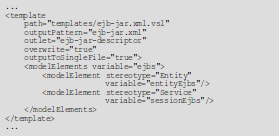
\includegraphics[width=380pt,height=180pt]{files/imgs/apendice-cartucho-novo-00001.png}
	\caption{Exemplo de uso da propriedade modelElement.}
	\label{exemplo_model_element}
\end{figure}

No exemplo acima, todos os elementos de modelo com os estereótipos
\texttt{<<Entity>>} e \texttt{<<Service>>} estarão disponíveis para os Templates
Velocity sob as variáveis \textdollar{}entityEjbs e \textdollar{}sessionEjbs,
respectivamente. Mas também haverá uma variável \textdollar{}ejbs que estará
disponível para os Templates Velocity, contendo tanto os elementos de modelo com
o esteriótipo \texttt{<<Entity>>}, quanto os elementos de modelo com o
esteriótipo \texttt{<<Service>>}.

\item <type/> - Este elemento opcional e aninhado com o elemento
<modelElement/>, é utilizado para informar ao Template Velocity qual elemento de
modelo deverá ser processado. Os elementos de modelo a serem processados serão
aqueles que estiverem associados à Metafacade definida pelo atributo name. Não é
necessário utilizar tal elemento caso o atributo stereotype do elemento
<modelElement/> esteja definido. Possui os seguintes atributos:

\begin{itemize}
  \item name(*) - O nome completo da classe para o Metafacade.
\end{itemize}

\item <property/> - Este elemento opcional e aninhado com o elemento <type/>, é
utilizado para informar ao Template Velocity qual elemento de modelo deverá ser
processado. Os elementos de modelo a serem processados serão aqueles que
estiverem associados à Metafacade definida pelo atributo name do elemento
<type/> acima, e caso esta Metafacade associada possua uma das propriedades
definidas por este elemento. Posui os seguintes atributos:

\begin{itemize}
  \item name(*) - O nome da propriedade para o Metafacade.
  \item value - O valor da propriedade para o Metafacade.
\end{itemize}

É importante atentar para o fato de que não é necessário especificar uma valor
para uma propriedade. Assim, caso o atributo value não seja especificado, a
propriedade precisa apenas ser válida: seja não-nula, possua um ou mais
elementos caso seja uma coleção ou seja verdadeira caso seja um tipo boolean.

Obs.: Atributos com o símbolo (*) são obrigatórios.

\subsection{Criando o arquivo de configuração do perfil do cartucho}
Crie no diretório \texttt{META-INF > andromda}, o arquivo \texttt{profile.xml}.
Este arquivo \texttt{XML} é reponsável por registrar os estereótipos e valores
etiquetados que serão usados pelo cartucho na interpretação do modelo. O arquivo
possui as seguintes \texttt{tags}:

\begin{itemize}
  \item <profile> - Raiz da configuração, deve englobar todas as demais tags.
  \item <documentation> - Descrição do que é o cartucho, seu intuito e demais
  informações que se julgue necessárias.
  \item <elements> - Tag que engloba a lista de elementos (estereótipos e
  valores etiquetados) a serem definidos.
  \item <elementGroup> - Devendo ser colocada dentro de <elements>, esta tag
  nos permite criar grupos de elementos definidos dentro de si e a usaremos para
  separar os elementos de acordo com o seu tipo. Esta tag possui uma propriedade
  \texttt{`name`}, usada para definir o nome do grupo criado (Ex.: Stereotypes).
  \item <element> - Devendo ser colocada dentro de um <elementGroup>, esta tag
  define um elemento a ser usado no modelo. Tem suas propriedades definidas com
  outras tags dentro de si. Cada elemento deve conter dentro de si as seguintes
  tags:
  \begin{enumerate}
    \item <documentation> - Descrição sobre o estereótipo sendo registrado.
    \item <value> - Valor, em texto, associado àquele estereótipo.
    \item <appliedOnElement> - Tipo de elemento \texttt{UML} ao qual tal
    estereótipo deve ser aplicado. Se queremos que ele só seja aplicado a
    classes, por exemplo, definiremos 
    `\texttt{<apliedOnElement>class<apliedOnElement/>}`.
  \end{enumerate}
\end{itemize}

\subsection{Criando arquivo de Configuração dos metafacades do cartucho}

\subsection{Criando o arquivo de configuração do Namespace do cartucho}
Crie no diretório \texttt{META-INF > andromda}, o arquivo
\texttt{namespace.xml}. Este arquivo \texttt{XML} é responsável por registrar as
propriedades e variáveis globais que estarão disponíveis para os templates do
cartucho, bem como registrar os componentes do mesmo. O arquivo é composto das
seguintes tags:

	\begin{itemize}
	  \item <namespace> - Raiz da configuração, devendo englobar todas as tags
	  seguintes. Possui o atributo \texttt{name}, que define o nome do namespace
	  que se está definindo.
	  \item <components> - Define um conjunto de componentes de configuração a
	  serem registrados como parte do cartucho. Deve englobar as tags <component>
	  \item <component> - Registra um componente de configuração do cartucho.
	  Usaremos esta tag para registr os outros arquivos de configuração
	  anteriormente criados. Possui o atributo \texttt{name}, que define o nome do
	  componente, devendo ser preenchido com o mesmo nome do arquivo, sem a
	  extensão, ou seja, para o arquivo \texttt{cartridge.xml}, definiremos
	  \texttt{`name`=`catridge`}.
	  \item <path> - Define o caminho onde está localizado um componente de
	  configuração, devendo, portanto, ser definida dentro da tag <component>. É
	  importante notar que o caminho é definido considerando novo-cartuco/src como
	  a raiz do projeto, não devendo este caminho ser especificado. Para definir o
	  path para o arquivo \texttt{cartridge.xml}, que criamos no caminho,
	  novo-cartuco/src/META-INF/andromda, basta definir \texttt{<path>
	  META-INF/andromda/profile.xml}.
	  \item <properties> - Define um conjunto de propriedades do cartucho.
	  \item <propertyGroup>	- Define um grupo de propriedades, agrupadas
	  logicamente de acordo com o seu intuito. Deve conter obrigatoriamente um
	  atributo \texttt{name}, que define o nome do grupo sendo definido. Dentro
	  desta tag, serão definidas as propriedades referentes a tal grupo e,
	  opcionalmente, uma tag <documentation>, com alguma descrição sobre tal grupo 
	  de propriedades. Deve ser definida dentro da tag <properties>.
	  \item <property> - Define uma propriedade do cartucho. Cada propriedade
	  funciona como uma variável `global` do cartucho, acessível a todos os seus
	  templates. Uma propriedade deve ter, obrigatoriamente, o atributo `name`, que
	  define o nome daquela propriedade, e, opcionalmente, o atributo booleano
	  `required`, que determina se tal propriedade precisa ter um valor definido
	  para si no arquivo \texttt{XML} de configuração do \texttt{AndroMDA}
	  (\texttt{andromda.xml}). Caso `required` seja definido como \texttt{true}, o
	  AndroMDA emitirá uma warning caso a tal propriedade não tenha um valor
	  definido para si. Além disso, pode-se configurar propriedades adicionais em
	  uma <property>, definindo dentro dela as seguintes tags (nenhuma delas
	  obrigatória):
	  \begin{enumerate}
	    \item <default> - Valor default para tal propriedade.
	    \item <documentation> - Descrição da propriedade sendo definida.
	  \end{enumerate}

	\end{itemize}

\section{Criando os Templates Velocity}
O processo de criação dos Templates Velocity é bastante simples. Basicamente
precisamos criar para cada elemento <template/> definido no descritor de
configuração do cartucho (andromda-cartridge.xml), um arquivo VSL
correspondente. (Para maiores informações sobre Templates Velocity veja o Anexo
3 - Templates Velocity User Guide.) Veja abaixo um exemplo de arquivo VSL. Este
Template Velocity é utilizado para gerar um arquivo de propriedades para o
Struts Framework, definindo os nomes dos campos de formulários, assim como os
títulos das páginas a partir dos elementos de modelo.

\begin{figure}[H]
	\centering
	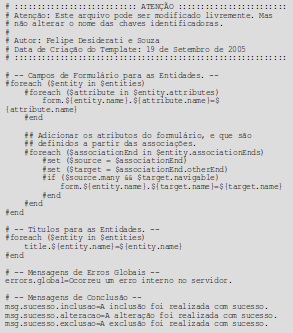
\includegraphics[width=280pt,height=260pt]{files/imgs/apendice-cartucho-novo-00005.png}
	\caption{Exemplo de Arquivo Velocity.}
	\label{exemplo_velocity}
\end{figure}

\end{enumerate}